% !TeX encoding = UTF-8
% Use XeLaTeX to compile it
%
% Эта работа распространяется на условиях лицензии Creative Commons Attribution-Noncommercial-Share Alike 3.0 New Zealand License.
% Краткое описание лицензии есть тут: http://creativecommons.org/licenses/by-nc-sa/3.0/nz/deed.ru
% Полное — там же.
% Эту книгу можно невозбранно распространять и изменять, но только соблюдая следующие условия:
% сохраняя лицензию и не вводя дополнительных ограничений, бесплатно
% и указывая авторство как оригинальной части, так и изменённой.
% Автор оригинального английского текста — Jason R Briggs http://jasonrbriggs.com/
% Автор перевода — Егор Кочетов <Egor.Kochetoff@gmail.com>
%
% This work is licensed under the Creative Commons Attribution-Noncommercial-Share Alike 3.0 New Zealand License.
% To view a copy of this license, visit http://creativecommons.org/licenses/by-nc-sa/3.0/nz
% or send a letter to Creative Commons, 171 Second Street, Suite 300, San Francisco, California, 94105, USA.
%

\chapter{Черепахи и другие медленные создания}\index{черепашка}\label{ch:turtles}

Есть нечто общее между черепахами из реального мира и черепахой в Питоне. В реальном мире черепаха — это (иногда) зелёная рептилия, которая движется очень медленно и носит на себе свой дом. В мире Питона всё почти так же: черепаха — это маленькая чёрная стрелочка, которая очень медленно ползает по экрану. Правда, с домиком у этой стрелочки не сложилось.

Вообще, черепашка в Питоне оставляет за собой след, так что она похожа больше на улитку, чем на черепаху. Но «черепаха» звучит более гордо, так что модуль в Питоне называется именно так. Можно представлять себе черепаху, зажавшую в зубах маркер и рисующую, пока ползёт.

Давным-давно, в тёмные старые времена люди придумали язык программирования Лого (Logo). Это был язык для управления роботом-черепашкой Ирвингом. Со временем черепашка превратилась из робота, ползающего по полу, в маленькую стрелочку, перемещающуюся по экрану.

\btw{Что, кстати, показывает нам, что с развитием технологии не всегда всё улучшается. Маленькая робот-черепашка на полу была бы куда как забавнее.}

В Питоне есть модуль\footnote{Про модули подробно поговорим мы чуть позже, а пока просто стоит иметь в виду, что модуль — это что-то, что можно использовать в своей программе, набор разных функций.} \code{turtle} (черепаха), и он в целом похож на язык Лого. Только Лого ничего, кроме черепашки, и не умеет, а Питон умеет ещё много всего другого. Модуль \code{turtle} полезен, чтобы понять, как компьютер рисует изображение на экране.

Ладно, давай теперь просто посмотрим, как же этот модуль работает. Во-первых, его надо «импортировать», то есть сказать Питону, что он нам нужен:

\begin{listing}
\begin{verbatim}
>>> import turtle
\end{verbatim}
\end{listing}

Потом нам надо создать «холст» для рисования — смысл тот же, что и в реальном холсте, которым пользуются художники. Холст будет нужен, чтобы на нём рисовать. Мы создадим пустой:

\begin{listing}
\begin{verbatim}
>>> t = turtle.Pen()
\end{verbatim}
\end{listing}

Тут мы вызываем функцию \code{Pen}\index{черепашка!Pen} модуля \code{turtle}, и она автоматически создаёт холст (\emph{canvas} по-английски). Вообще, функция — это что-то вроде маленькой программы, то есть кусочек кода, который можно использовать много раз (подробно функции мы обсудим потом). В данном случае функция \code{Pen} \emph{возвращает} нам черепашку, то есть результат этой функции — черепашка, к которой мы приклеиваем переменную \code{t}. Результатом этого кода должна быть картинка наподобие \ref{fig10}.

\begin{figure}
\begin{center}
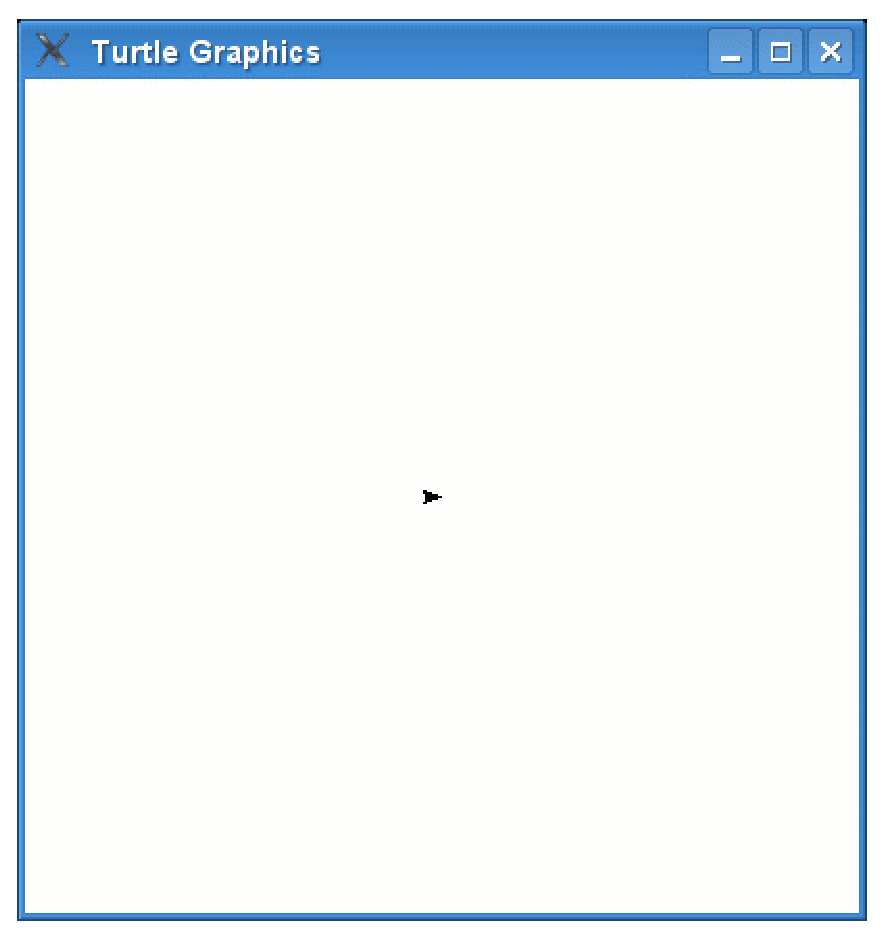
\includegraphics[width=72mm]{../en/figure10.eps}
\end{center}
\caption{Стрелочка, изображающая черепаху}\label{fig10}
\end{figure}

\btw{Да, эта маленькая стрелочке посреди экрана — действительно черепаха. И да, на черепаху она внешне не похожа примерно ничем.}

Этой черепахе можно отправлять инструкции, используя функции созданного объекта \code{t}. Вот, например, можно попросить черепаху продвинуться вперёд, туда, куда показывает стрелочка. Для этого есть функция \code{forward}, в скобках которой надо указать, на сколько точек на экране продвинуться. Например, чтобы подвинуть черепаху вперёд на 50 точек (и нарисовать линию длиной 50 точек), нужно выполнить такую команду:

\begin{listing}
\begin{verbatim}
>>> t.forward(50)
\end{verbatim}
\end{listing}

И в результате должно получиться как-то так:~\ref{fig11}.

\begin{figure}
\begin{center}
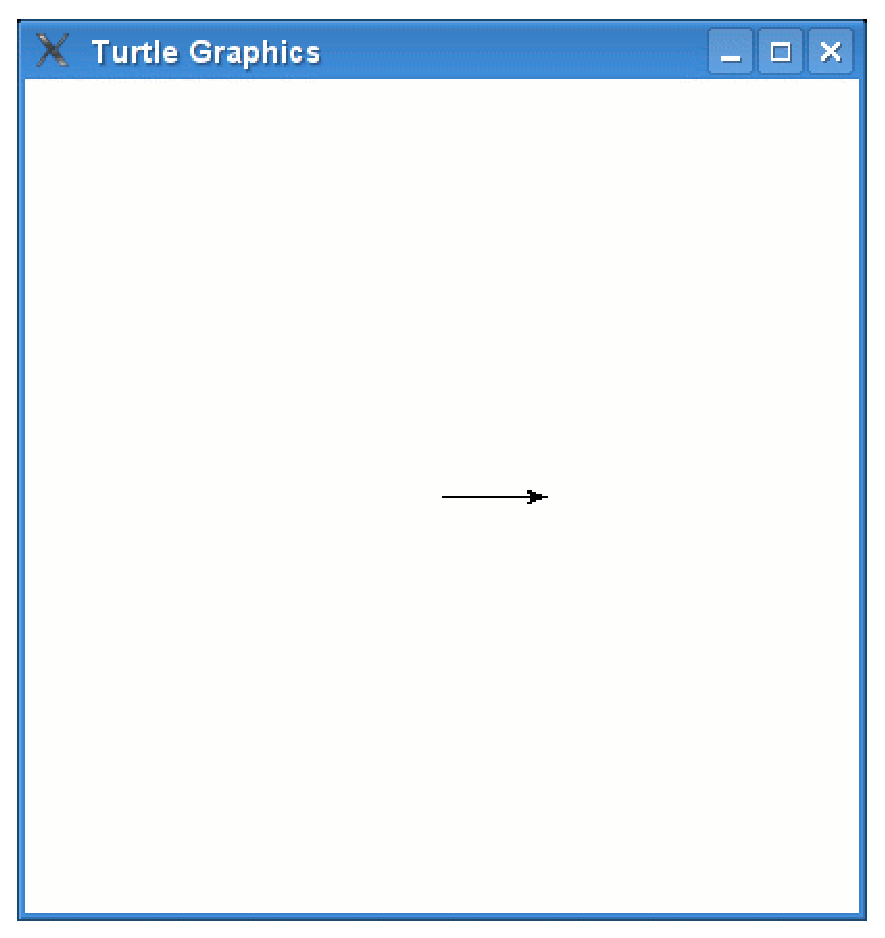
\includegraphics[width=72mm]{../en/figure11.eps}
\end{center}
\caption{Черепашка нарисовала линию.}\label{fig11}
\end{figure}

С точки зрения черепахи, она прошла вперёд 50 шагов. А мы бы сказали, что она прошла 50 точек по экрану.

\btw{И что это за точки такие?}

Всё на экране компьютера состоит из отдельных маленьких точек, каждая из которых окрашена в свой цвет. Обычно их называют пикселями, чтобы не путать ни с какими другими точками, и так я и буду дальше делать. Все программы на компьютере, все игры заставляют точки на экране окрашиваться в разные нужные цвета. Эти отдельные точки можно увидеть, вооружившись лупой. Если сильно увеличить линию, нарисованную черепахой, то можно увидеть, что это много квадратных точек, оказавшихся рядом, как на картинке \ref{fig12}.

\begin{figure}
\begin{center}
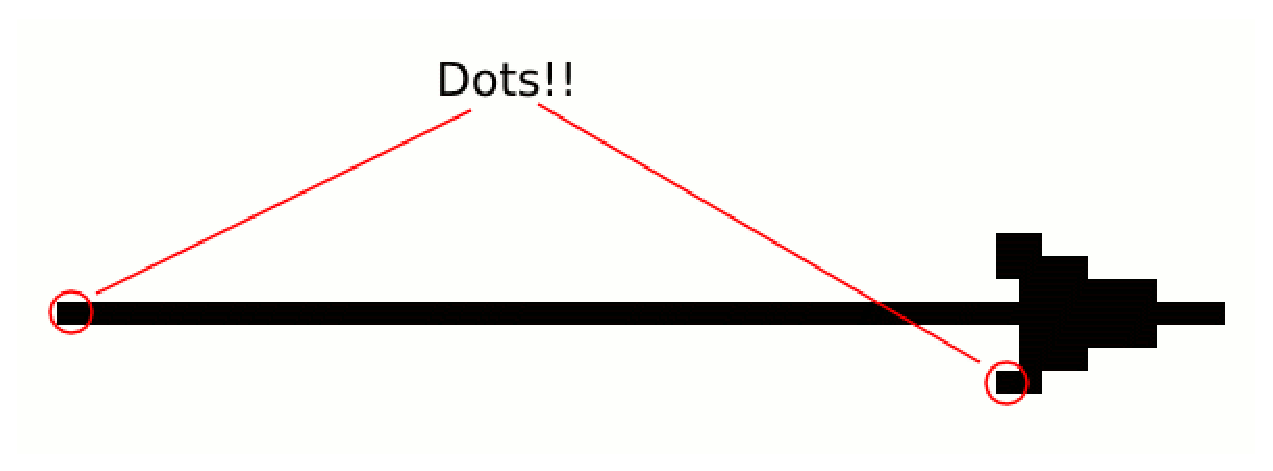
\includegraphics[width=72mm]{../en/figure12.eps}
\end{center}
\caption{Сильно увеличенные линия и стрелочка.}\label{fig12}
\end{figure}

В следующих главах мы ещё вспомним про пиксели, они нам пригодятся.

Вернёмся к черепашке. Её ещё можно попросить повернуть направо\index{черепашка!поворот направо} и налево\index{черепашка!поворот налево}.

\begin{listing}
\begin{verbatim}
>>> t.left(90)
\end{verbatim}
\end{listing}

Эта команда говорит черепашке повернуть налево на 90 градусов (то есть против часовой стрелки). Если ты ещё не знаешь про градусы\index{градусы} и как ими меряют углы, то это можно представить себе вот как. На рисунке \ref{fig13} есть циферблат от часов.

\begin{figure}
\begin{center}
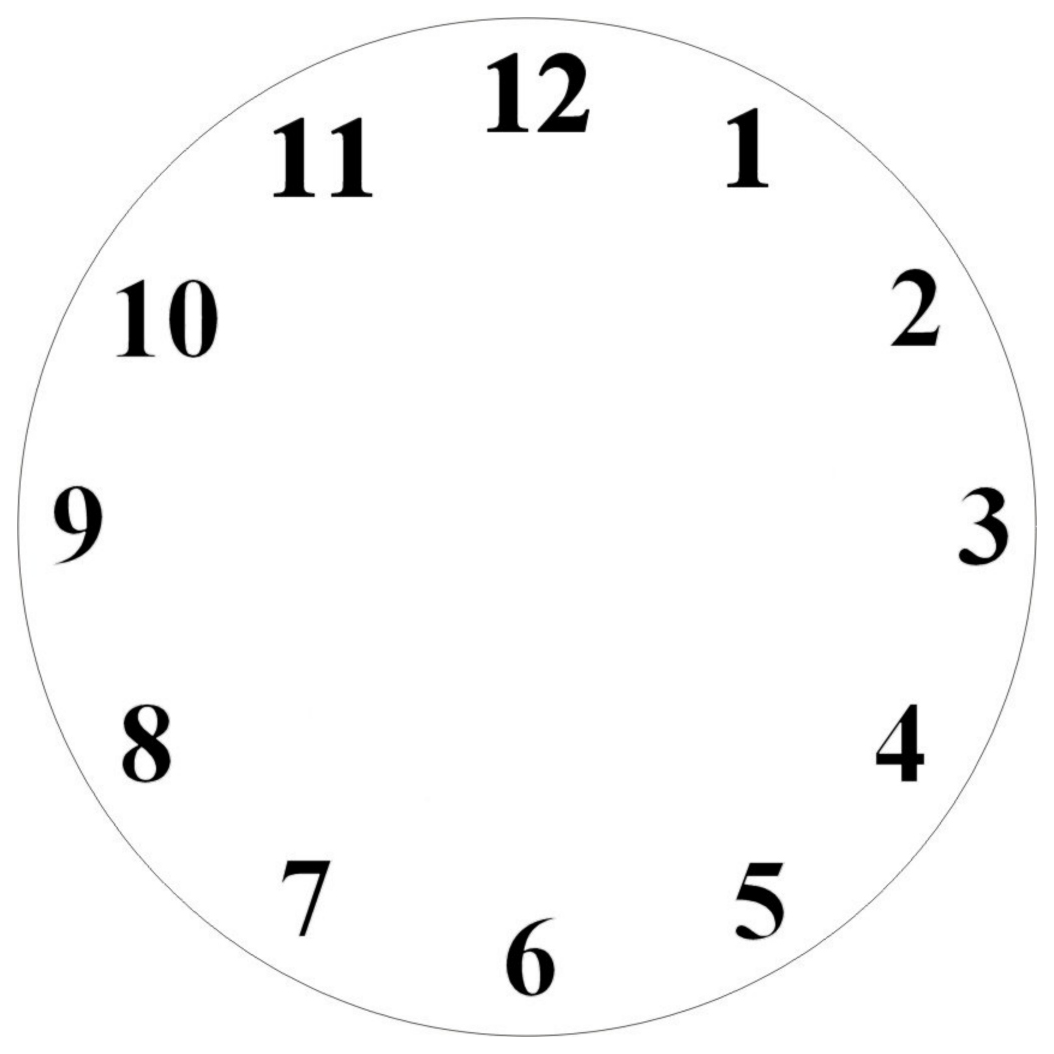
\includegraphics[width=52mm]{../en/figure13.eps}
\end{center}
\caption{Циферблат с отметками часов}\label{fig13}
\end{figure}

На циферблате по кругу написаны числа от 1 до 12 (или до 60, если там написаны минуты). Так вот градусы пишутся так же по кругу, только всё умножается на 30. Вместо цифры 3 — 90° (90 градусов), вместо шести — 180°, как на рисунке \ref{fig14}. А черепашка как будто стоит в центре циферблата и смотрит в сторону нуля, наверх.

\begin{figure}
\begin{center}
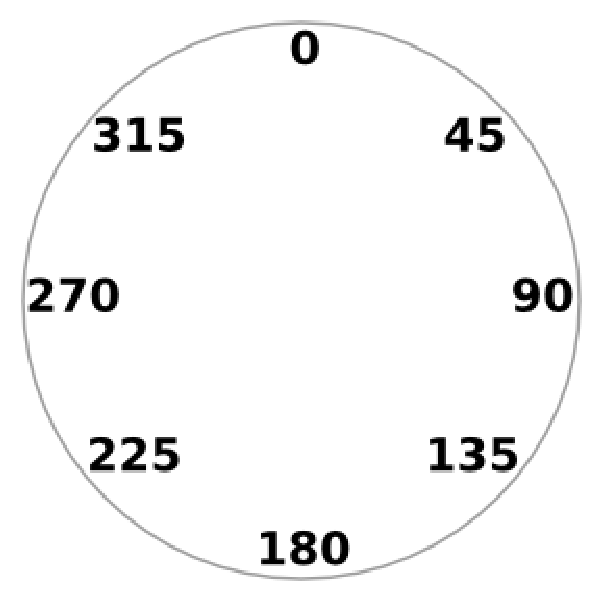
\includegraphics[width=52mm]{../en/figure14.eps}
\end{center}
\caption{Градусы.}\label{fig14}
\end{figure}

И что происходит, когда мы отдаём команду \code{left(90)}?

Если встать, поднять руку ровно в сторону и показать туда, то чтобы повернуться лицом в ту сторону, в которую ты показываешь, нужно повернуться как раз на 90 градусов. Если показывать правой рукой, то на 90° вправо, левой рукой — на 90° влево. Так же и черепашка в питоне поворачивается туда, где её правый бок или левый. При этом голова черепашки остаётся на месте (рисует она как раз маркером, зажатым в зубах), так что функция \code{t.left(90)} приводит к тому, что есть на рисунке \ref{fig15}. Черепашка ползла вправо и повернула вверх.

\begin{figure}
\begin{center}
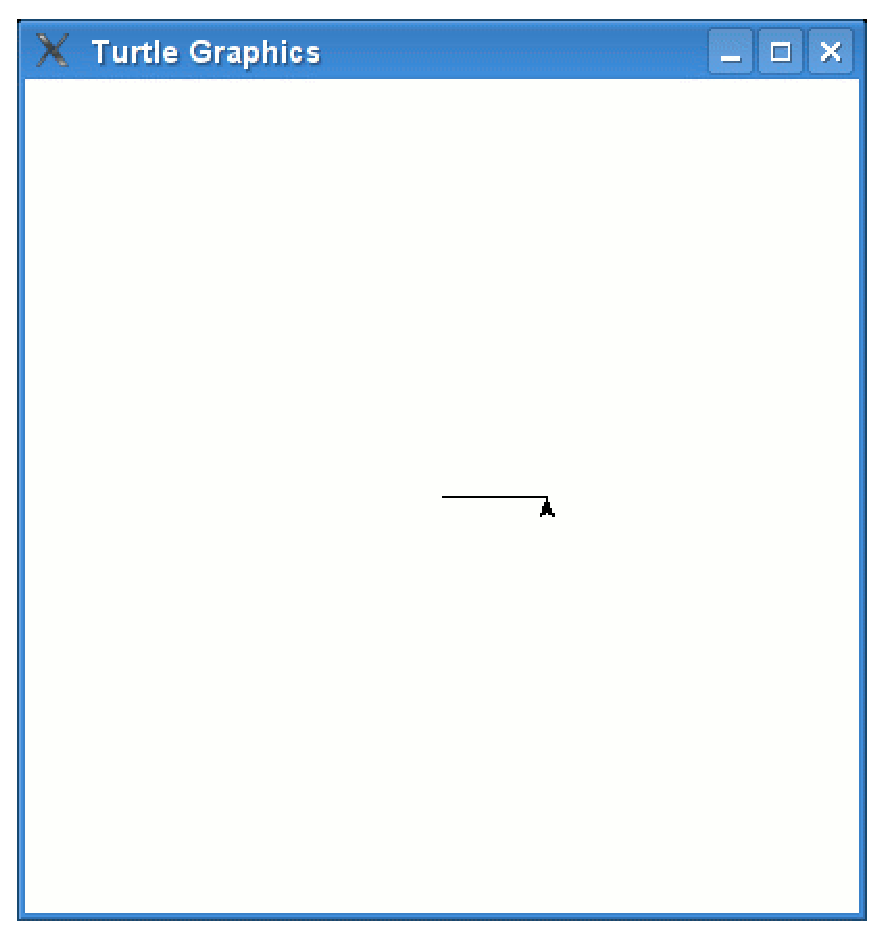
\includegraphics[width=72mm]{../en/figure15.eps}
\end{center}
\caption{Черепашка, повернувшая налево.}\label{fig15}
\end{figure}

Давай теперь посмотрим, как все эти команды работают вместе:

\begin{listing}
\begin{verbatim}
>>> t.forward(50)
>>> t.left(90)
>>> t.forward(50)
>>> t.left(90)
>>> t.forward(50)
>>> t.left(90)
\end{verbatim}
\end{listing}

На экране черепашка нарисовала квадрат и остановилась, глядя в ту же сторону, что и в начале пути, как на рисунке \ref{fig16}.

\begin{figure}
\begin{center}
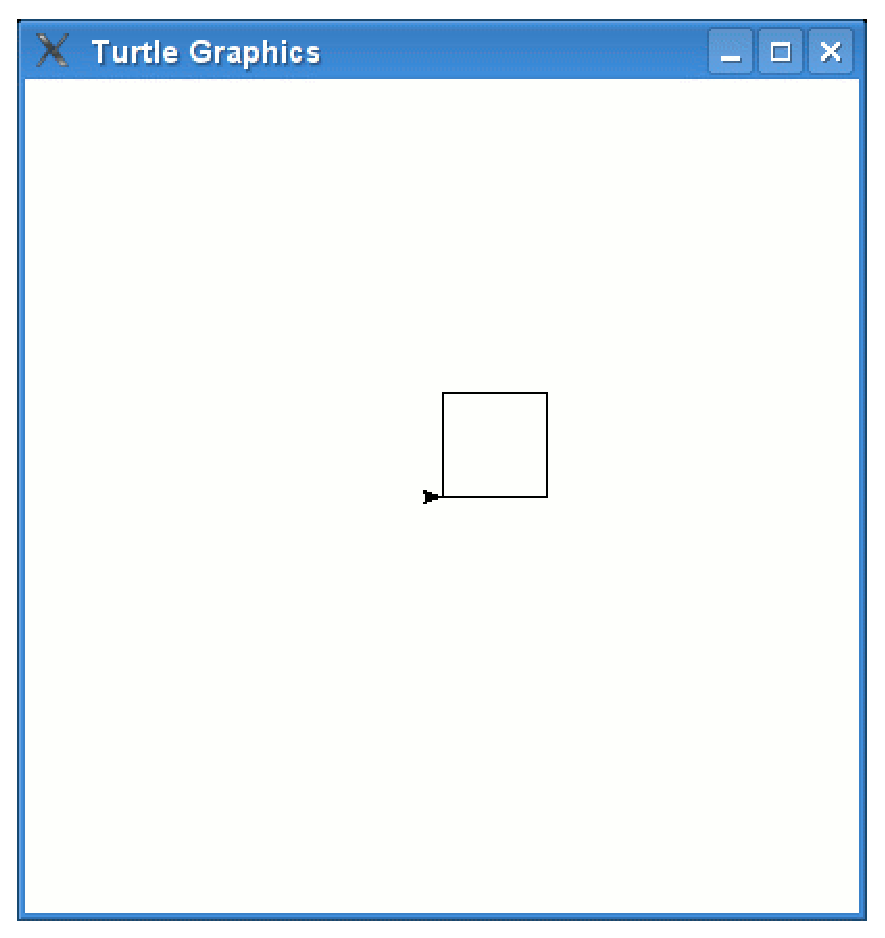
\includegraphics[width=72mm]{../en/figure16.eps}
\end{center}
\caption{Квадрат нарисовался.}\label{fig16}
\end{figure}

Можно взять и очистить весь холст, воспользовавшись функцией \code{clear}\index{черепашка!очистить} (что как раз и переводится как «очистить»):

\begin{listing}
\begin{verbatim}
>>> t.clear()
\end{verbatim}
\end{listing}

Есть и другие полезные функции, применимые к черепашке. Например, \code{reset}\index{черепашка!reset}: тоже очищает экран и ещё перемещает черепашку в начальное положение. Ещё есть функция \code{backward}, которая говорит черепашке двигаться назад (при этом направление её взгляда не меняется, она просто пятится). Функция \code{right} говорит черепашке повернуть направо; функция \code{up}\index{черепашка!прекратить рисовать} говорит ей оторвать маркер от холста, то есть перестать рисовать при движении: не всё можно нарисовать, если рисовать при каждом движении, иногда нужно просто переместиться. Есть и функция \code{down}\index{черепашка!начать рисовать}, которая говорит ей обратно опустить маркер на холст и снова рисовать, пока она перемещается. Все эти функции вызываются таким же образом, как в примерах выше:

\begin{listing}
\begin{verbatim}
>>> t.reset()
>>> t.backward(100)
>>> t.right(90)
>>> t.up()
>>> t.down()
\end{verbatim}
\end{listing}

В следующих главах мы ещё воспользуемся услугами черепашки.

\section{Что ещё попробовать}

\btw{В этой главе мы познакомились с маленькой черепашкой, которая нарисовала нам немного линий, поворачиваясь направо и налево. Ещё мы обсудили градусы, которые здорово похожи на числа на циферблате часов.}

\subsection*{Упражнение 1}
Создай холст, используя функцию \code{Pen}, и нарисуй там прямоугольник.

\subsection*{Упражнение 2}
Создай холст, используя функцию \code{Pen}, и нарисуй там треугольник.

\subsection*{Упражнение 3*}
Создай холст, используя функцию \code{Pen}, и нарисуй там домик, как на рисунке \ref{fighouse}, не отрывая маркер от холста (не пользуясь функцией \code{up}). Это упражнение сложнее предыдущих и может не получиться без посторонней помощи, ничего страшного\footnote{Чтобы всё получилось, нужно иметь в виду, что может понадобиться повернуть на 45 или 135 градусов и что если стороны домика длиной 100 точек, то косые линии будут длиной примерно 71 и 141 точка.}.

\begin{figure}
\begin{center}
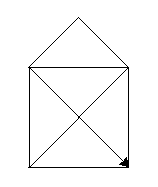
\includegraphics[width=72mm]{03.house.png}
\end{center}
\caption{Домик, который нарисовали, не отрывая карандаш от бумаги.}\label{fighouse}
\end{figure}

\newpage
